\documentclass[border=4pt,tikz]{standalone}
\usepackage{tikz}
\usetikzlibrary{positioning, arrows.meta}

\begin{document}
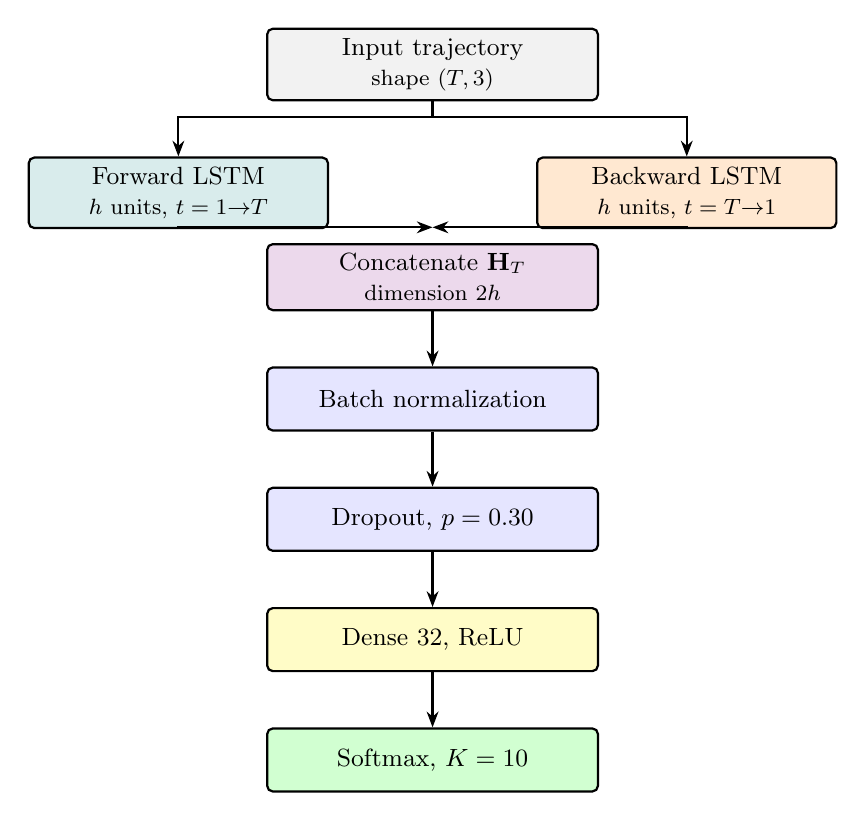
\begin{tikzpicture}[
    node distance = 7mm,
    every node/.style = {font=\small},
    layer/.style    = {rectangle, rounded corners=2pt, draw, thick,
                       minimum width=42mm, minimum height=8mm,
                       align=center, fill=gray!10},
    lstmF/.style    = {layer, fill=teal!15,   minimum width=38mm},
    lstmB/.style    = {layer, fill=orange!18, minimum width=38mm},
    concat/.style   = {layer, fill=violet!15},
    reg/.style      = {layer, fill=blue!10},
    dense/.style    = {layer, fill=yellow!22},
    outnode/.style  = {layer, fill=green!18},
    arr/.style      = {-{Stealth[length=2mm]}, thick}
]
\node[layer] (in)   {Input trajectory \\ \footnotesize shape $(T, 3)$};
\node[lstmF, below left  = 7mm and -8mm of in] (fw) {Forward LSTM \\ \footnotesize $h$ units, $t=1{\to}T$};
\node[lstmB, below right = 7mm and -8mm of in] (bw) {Backward LSTM \\ \footnotesize $h$ units, $t=T{\to}1$};
\node[concat, below = 18mm of in]              (cc) {Concatenate $\mathbf{H}_T$ \\ \footnotesize dimension $2h$};
\node[reg,   below = of cc]                    (bn) {Batch normalization};
\node[reg,   below = of bn]                    (dp) {Dropout, $p=0.30$};
\node[dense, below = of dp]                    (de) {Dense $32$, ReLU};
\node[outnode, below = of de]                    (sm) {Softmax, $K=10$};

\draw[arr] (in.south) -- ++(0,-2mm) -| (fw.north);
\draw[arr] (in.south) -- ++(0,-2mm) -| (bw.north);
\draw[arr] (fw.south) |- ([yshift=2mm]cc.north);
\draw[arr] (bw.south) |- ([yshift=2mm]cc.north);
\draw[arr] (cc) -- (bn);
\draw[arr] (bn) -- (dp);
\draw[arr] (dp) -- (de);
\draw[arr] (de) -- (sm);
\end{tikzpicture}
\end{document}